\chapter{Execution Monitoring}

Unicon's execution monitoring facilities allow the user to execute a Unicon
program under the observation of one or more monitoring programs, also
written in Unicon.  This chapter presents the monitoring architecture and a
standard execution monitoring scenario, followed by details of the language
features involved.  This chapter is based on ``Program Monitoring and
Visualization'' \cite{Jeff99}, which has many additional examples.

\section{Monitor Architecture}

The monitoring facilities components are summarized in Figure 9-1.
Many of these components are general-purpose language features that are
useful independent of execution monitoring.

\begin{center}
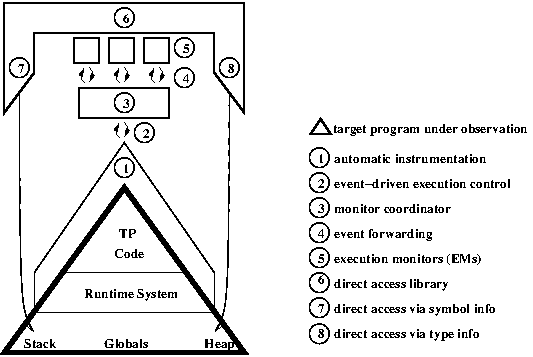
\includegraphics[height=2.8in]{alamarch.png}
\end{center}

{\sffamily\bfseries Figure 9-1:}
{\sffamily The Alamo architecture}

\bigskip

\subsection{Monitor Terminology}

The terminology used in discussing Unicon's execution monitoring
architecture relates to events and the linguistic features associated with
them.



\begin{list}{}{\itemsep 7pt}
\item [{\bf Dynamic loading}] --- The ability to load multiple programs
	into a shared execution environment supports
	monitor access to target program data.
	{\em Dynamic linking\/} is {\em not\/} desirable in the
	context of execution monitoring; the names in the
	monitor are distinct from those in the target program. 
	\index{dynamic loading}
\item [{\bf Synchronous execution}] --- The monitor and target program execute
	independently, but not concurrently.  This allows the monitor
	to control target program execution using a simple programming model.
	Unicon's {\em co-expression\/} data type is used to support the
	relationship between monitor and target program.
	\index{synchronous execution|see{coroutine}}
\item [{\bf High-level instrumentation}] --- Information
	about program execution is available to the monitor from
	locations in the language runtime system that are coded to report
	significant events.  This obviates the need for, and
	offers higher performance than target program
	instrumentation.  The runtime system instrumentation is a
	generalization of an earlier special-purpose
	monitoring facility oriented around dynamic memory allocation
	and reclamation \cite{Town89}.
	It also supercedes Icon and Unicon's procedure
	tracing mechanism.
	\index{automatic instrumentation}
\item [{\bf Events}] --- 
	The primary language concept added in order to support execution
	\index{event}
	monitoring is an {\em event\/}.  An event is the smallest unit of
	execution behavior that is observable by a monitor.  In practice, an
	event is the execution of an instrumentation point in the code
	(a {\em sensor\/}) \index{sensor}
	that is capable of transfering control to the monitor.
	\index{instrumentation}
	This definition limits events to those aspects of program behavior
	that are instrumented in the language runtime system or the program
	itself. If instrumentation
	does not exist for an aspect of program behavior of interest, it is
	often possible to monitor the desired behavior by means of other
	events. In the present implementation, for example, no instrumentation
	exists for file input and output.  If an EM wishes to monitor I/O
	behavior, it can monitor function and operator events and act on
	those functions and operators that relate to input and output.
	A similar example involving the monitoring of Icon's built-in
	string scanning functions is presented in [Jeffery99]

	In Unicon, events occur whether
	they are monitored or not, and each event may or may not be observed
	by any particular monitor.  This definition is useful in a
	multi-monitor environment, in which EMs are not coupled with the
	instrumentation and multiple EMs can observe a TP's execution.

\item [{\bf Event codes and values}] --- 
	From the monitor's perspective, an event has two components: an
	\index{event!code}\index{event!value}
	{\em event code\/} and an {\em event value\/}.  The code is
	generally a one-character string describing what type of event
	has taken place.  For example, the event code {\tt C} denotes a
	procedure call event.  Event codes all have associated symbolic
	constants used in program source code.  For example the mnemonic for a
	procedure call event is {\tt E\_Pcall}.  These constants are available
	to programmers as part of a standard event monitoring library
	described below.\index{E\_Pcall@{\tt E\_Pcall}}

	The event value is an Icon value associated with the event.  The
	nature of an event value depends on the corresponding event code.
	For example, the event value for a procedure call event is an
	Icon value designating the procedure being called, the event value for
	a list creation event is the list that was created, the event value
	for a source location change event is the new source location, and so
	forth.  Event values can be arbitrary Icon structures with pointer
	semantics; the EM accesses them just like any other source language
	value.\index{access!structure}

\item [{\bf Event reports}] --- 
	The number of events that occurs during a program execution is
	extremely large---large enough to create serious performance problems
	in an interactive system.  Most EMs function effectively on a
	small fraction of the available events; the events that an EM uses
	are said to be {\em reported\/} to the EM.  An {\em event report\/}
	results in a transfer of control from the TP to the EM.  Efficient
	support for the selection of appropriate events to report and the
	minimization of the number of event reports are primary concerns.
	\index{event!report}


\item [{\bf Event masks}] --- 
	A monitor controls the target program by means of this
	dynamic form of filtering events.
	\index{event!mask}\index{filtering}\index{event mask}
	An event mask is a set that
	describes the execution behavior of interest to the monitor.
	Because event codes are one-letter strings,
	the {\em cset\/} data type is used for event masks.
	Csets are represented internally by bit
	vectors, so a cset membership test is very efficient compared to
	the set data type, whose membership test is a hash
	table lookup.\index{cset!event mask}\index{character set!event mask}

	Event masking allows the monitor to specify which
	events are to be reported and to change the specification at runtime.
	Events that are of no interest to the execution
	monitor are not reported and do not impose unreasonable
	execution cost.
	When a monitor starts or resumes execution of the program being
	monitored, the monitor selects
	a subset of possible event codes from which to receive its first
	report.  The program executes until an event occurs with a selected
	code, at which time the event is reported.  After the monitor has
	finished processing the report, it transfers control back to the
	program, again specifying an event mask.  Dynamic event masking
	enables the monitor to change the event mask in between event reports.


	When an event report transfers control from TP to EM, the two
	components of the event are supplied in the Icon keywords
	{\tt \&eventcode} and {\tt \&eventvalue}, respectively.
	\index{event!code}\index{event!value}
	As discussed earlier, these
	keywords are special global variables that are given their values by
	the runtime system during an event report, rather than by explicit user
	assignment.  The monitor then can act upon the event
	based on its code, display or manipulate its value, etc.
\end{list}


\subsection{Standard Execution Monitoring Scenario}

The following scenario presents the relationship between execution monitors
and target program in its simplest form.  More sophisticated relationships
between the monitor and target program, such as running many monitors on a
single target program via a monitor coordinator, are described in ``Program
Monitoring and Visualization'' [Jeffery99].  In addition, the expected user
and range of program behavior observable using these monitoring facilities
are characterized.

\subsubsection*{Scenario Definitions}

\begin{tabular}{m{0.95in} m{4.75in}}
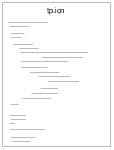
\includegraphics[width=0.65in,height=0.85in]{tp.png} &
{\bf target program (TP)} ---
The target program is the Unicon program under study, a translated Unicon
executable file.
Monitoring does not require that the TP be recompiled, nor that
the TP's source code be available, although some monitors make use of
program text to present information. \index{target program!Alamo} \\
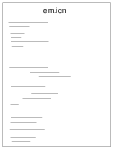
\includegraphics[width=0.65in,height=0.85in]{em.png} &
{\bf execution monitor (EM)} ---
An execution monitor is a Unicon program that collects and presents
information from an execution of a TP. \index{execution monitor!Alamo} \\
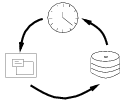
\includegraphics[width=0.6in,height=0.6in]{behave.png} &
{\bf program behavior} ---
Program behavior denotes the results of executing the TP.  Behavior is meant
in a general sense
that includes program output, execution time, and the precise sequence
of actions that take place during execution. \index{program behavior} \\

\includegraphics[height=0.7in]{user.png} &
\ \linebreak {\bf user} --- In our standard
scenario, the user is a human capable of understanding the TP's execution
behavior.  The user must know the target language in order to make good use
of many EMs or to write a new
EM.  In general, the user need not necessarily be familiar with the TP's
source code. \index{user!Alamo} \\
\end{tabular}

\bigskip

Execution monitoring begins with a user who has questions about the behavior
of a TP (Figure 9-2). Typical questions relate to correctness or performance,
such as ``How is the result calculated?'' or ``What is taking so long?''.
Questions may be more general in nature if the user is just trying to
understand how a program works.

\begin{center}
  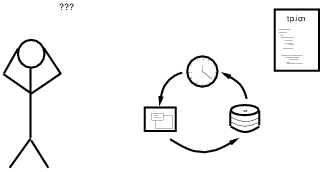
\includegraphics[height=1.7in]{scene1.png}
\end{center}
\vspace{-0.25cm}{\sffamily\bfseries Figure 9-2:}
{\sffamily Monitoring starts with a user, a program, and questions.}

\bigskip

Answers to important questions can be found by following the execution at
the source language level, but key behavior often depends upon language
semantics, implemented by the language runtime system.  In Figure 9-3,
{\tt iconx.c} denotes the set of files in the Unicon language runtime
system.\index{runtime system!Unicon} Many monitors can
provide useful information about runtime behavior even if the TP's source
code is not available.  Figure 9-3 could be elaborated to include
dependencies on the platform on which the program is running.

\begin{center}
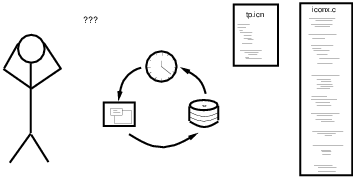
\includegraphics[height=1.7in]{scene2.png}
\end{center}

{\sffamily\bfseries Figure 9-3:}
{\sffamily Behavior depends on the language, not just the program.}

\subsubsection*{Selecting or Developing Appropriate Monitors}

Rather than focusing on one monolithic EM that attempts to accommodate
all monitoring tasks, the framework advocates development of a suite
of specialized EMs that observe and present particular aspects of a
TP's behavior.  The user is responsible for selecting an appropriate
EM or set of EMs that address the user's
concerns.\index{special purpose monitors}

If no available EM can provide the needed information,
the user can modify an existing EM or write a new one.  This end user
development of execution monitors is also useful when an existing EM
provides the needed information, but it is obscured by other
information; existing EMs can be customized to a particular problem.

\subsubsection*{Running the Target Program}

The user runs the TP, monitored by a selection of
EMs (Figure 9-4). General-purpose EMs provide an overall impression
of program behavior.  Visualization techniques enable the presentation
of a large amount of information and abstract away detail.
\index{run!program under monitor}

\begin{center}
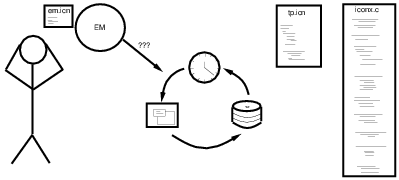
\includegraphics[height=1.7in]{scene3.png}
\end{center}

{\sffamily\bfseries Figure 9-4:}
{\sffamily EMs can answer questions about TP behavior.}

\bigskip

Obtaining specific information often requires that the user
interact with the EMs to control the TP's execution, either to increase
the amount of information presented during specific portions of
execution or to pause execution to examine details.
In order to provide this interactive control, EMs present
execution information as it happens during the TP's execution,
rather than during a postmortem analysis phase.
\index{user!interaction}\index{execution!control}\index{analysis!runtime}
\index{analysis!post mortem}

\subsection{Framework Characteristics}

The preceding scenario requires language support in several areas:
controlling a program's execution, obtaining execution information,
presenting large quantities of information, and interacting with the user.
To support these tasks, the framework provides synchronous shared address
multitasking and an event-driven execution control model.
\index{shared address} The first two of these features are the focus
of this chapter.

\subsubsection*{Multitasking}

In the monitoring execution model, in which an EM is a separate program
from the TP \index{execution model!multitasking}, the relationship is almost
that of two co-expressions, except that activations of the monitor are
implicit occurrences of events within the runtime system, rather than
expression results or explicit activations using the \texttt{@} operator.
Event reports are transfers of control to the monitor as well as the
primary source of execution information from a TP (Figure 9.5).

\begin{center}
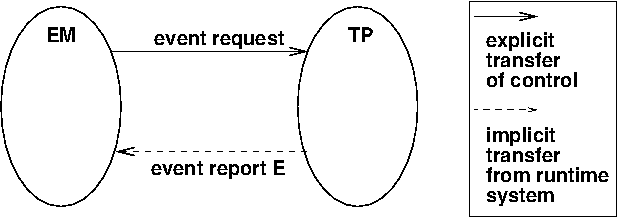
\includegraphics[width=2.8in,height=1.5in]{execinf.png}
\end{center}

{\sffamily\bfseries Figure 9-5:}
{\sffamily EM and TP are separately loaded coroutines}

\bigskip


Multitasking has the following benefits for monitoring: the EM and TP are
independent programs, the EM has full access to the TP, and the mechanism
accommodates multiple EMs.  These benefits are described in more detail
below.


\subsubsection*{Independence}

Because the EM and TP are separate programs, the TP need not be
modified or even recompiled in order to be monitored by an EM, and
EMs can be used on different target programs. By definition, execution
of tasks such as EMs and TPs is synchronous.  The TP is not
running when an EM is running, and vice versa.  This synchronous
execution allows EMs and TPs to be independent without introducing the
complexities of concurrent programming. In a concurrent context, each
thread might have a monitor, but the target thread and its associated
monitor are not concurrent --- and monitoring concurrent programs is not
yet supported by the implementation.
\index{independence!of EM and TP}\index{control flow}\index{callback}

Another degree of EM and TP independence is afforded by separate
memory regions; EMs and TPs allocate memory from separate heaps.
\index{memory regions!separate}\index{heap!EM separate from TP}
Memory allocation in the EM does not affect the allocation
and garbage collection patterns in the TP. Because Unicon is a type-safe
language with runtime type checking and no pointer data types, EMs
and TPs cannot corrupt each others' memory by accident; only code that
contains explicit references to another program's variables and data
can modify that program's behavior.
EMs can (and some do) modify TP values in arbitrary ways; the purpose
of separate memory regions is to minimize {\em unintentional\/} data
intrusion.


\subsubsection{Access}

An address space is a mapping from machine addresses to computer memory.
\index{address space}\index{access}
Within an address space, access to program variables and data is direct,
efficient operations such as single machine instructions.  Accessing
program variables and data from outside the address space is slow and
requires operating system assistance.

The EM and TP reside within the same address space.  This allows EMs to
treat TP data values in the same way as their own: EMs can access TP
structures using regular Unicon operations, compare TP strings with their own,
and so forth.
Because of the shared address space, the co-expression switch used
to transfer execution between EMs and TPs is a fast,
lightweight operation.  This is important because monitoring
requires an extremely large number of task switches compared to
typical multitasking applications.\index{context switch!lightweight}
\index{task switch}


\subsubsection{Multiple Monitors and Monitor Coordinators}

Unicon's dynamic loading capabilities allow simultaneous execution of
not just a single EM and a single TP, but potentially many EMs, TPs,
and other Icon programs in arbitrary configurations.  Although uses
for many such configurations can be found, one configuration merits
special attention when many specialized EMs are available: the
execution of multiple monitors on a single TP \index{dynamic loading}
(Figure 9-6, left).

\begin{center}
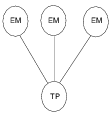
\includegraphics[height=2.0in]{multiems.png}
\hspace{1cm}
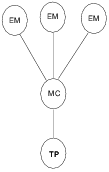
\includegraphics[height=2.8in]{mcover.png}
\end{center}

{\sffamily\bfseries Figure 9-6:}
{\sffamily Multiple EMs (left); EMs under a monitor coordinator (right)}

\bigskip

The difficulty posed by multiple monitors is not in loading the
programs, but in coordinating and transferring control among several
EMs and providing each EM with the TP execution information it
requires.  Since EMs are easier to write if they need not be aware of
each other, things are much simpler if EMs run under a
{\em monitor coordinator\/} (MC), a special EM that monitors a TP and
provides monitoring services
to one or more additional EMs (Figure 9-6, right).  EMs receiving an MC's
services need not be aware of the presence of an MC any more than a TP
need be aware of the presence of an EM.\index{monitor coordinators}

The virtual monitor interface provided by MCs makes adding a new monitor to
the system extremely easy.  A new monitor could conceivably be written,
compiled, linked, and loaded during a pause in the TP's execution. In
addition, constructing efficient MCs that provide high-level services is
another area of research that is supported within the Alamo Icon framework.
\index{virtual monitor}

\subsubsection*{Support for Dual Input Streams}

An EM typically has two primary input streams: the event stream from
the TP, and the input stream from the user (Figure 9-7).  Although
these two input streams are conceptually independent and may be
treated as such, for many EMs this unnecessarily complicates
the central loop that obtains event reports from TP---the EM must
also check its own window for user activity.\index{event stream!dual}
\index{input stream!dual}

\begin{center}
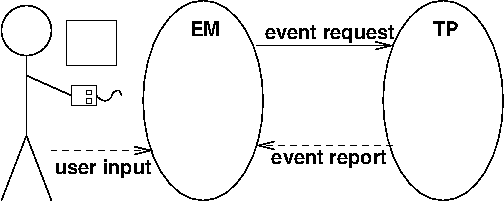
\includegraphics[width=3.0in,height=1.5in]{eventstr.png}
\end{center}

{\sffamily\bfseries Figure 9-7:}
{\sffamily Monitors have two input streams}

\bigskip


The runtime system instrumentation includes code that optionally
checks for EM input and reports it as an event by the execution
monitoring facility, instead of requiring that the EM explicitly check
the user input stream.  This simplifies EM control 
flow and improves EM performance.

\section{Obtaining Events Using {\tt evinit}}

A standard library called {\tt evinit} provides EMs with
a means of obtaining events.  Programs wishing to use the
standard library include a link declaration such as {\tt link
evinit}.\index{evinit library}
\index{library procedures!monitor}
In addition, monitors include a header file named {\tt evdefs.icn}
to obtain the symbolic names of the event codes.
\index{evdefs.icn@{\tt evdefs.icn}}

\subsection*{Setting Up an Event Stream}

\vspace{0.25pc}
\noindent
An EM first sets up a source of events; the act of monitoring then
\index{event!source}
consists of a loop that requests and processes events from the TP.
\index{EvInit@{\tt EvInit()}}
Execution monitoring is initialized by the procedure
{\tt EvInit(x{\em [,input,output,error]\/})}.  If {\tt x} is a string, it is
used as an icode file name in a call to the Unicon function {\tt load()}.
If {\tt x} is a list, its first argument is taken as the icode file name
and the rest of the list is passed in to the loaded function as the
arguments to its main procedure.
{\tt EvInit()} assigns the loaded
TP's co-expression value to EM's {\tt \&eventsource} keyword.
The {\tt input}, {\tt output}, and {\tt error} arguments are files
used as the loaded program's standard files.

EMs generally call the library procedure {\tt EvTerm()} when they complete,
passing it their main window (if they use one) as a parameter.
\index{EvTerm@{\tt EvTerm()}}
{\tt EvTerm()} informs the user that execution has completed and allows the
final screen image to be viewed at the user's leisure, waiting for the user to
press a key or mouse button in the window and then closing it.

The typical EM, and all of the EMs presented as examples in this
book, follow the general outline:\index{outline!of an EM}
\index{skeleton!of an EM} \index{template!of an EM}

%%%% \pagebreak
\iconcode{
     \$include \"evdefs.icn\" \\
     link evinit \\
     procedure main(arguments) \\
\>	EvInit(arguments) $\mid$ stop(\"can't initialize monitor\") \\
\>	\# ... initialization code, open the EM window \\
\>	\# ... event processing loop (described below) \\
\>	EvTerm() \\
     end
}
\noindent This template is generally omitted from program examples for
the sake of brevity.

\subsection*{\tt EvGet()}

Events are requested by an EM using the function {\tt EvGet(mask)}.
\index{EvGet@{\tt EvGet()}}
{\tt EvGet(mask)} activates the co-expression value of the keyword 
{\tt \&eventsource} to obtain an event whose code is a member of the
cset {\tt mask}.
{\tt mask} defaults to {\tt \&cset}, the universal set indicating all events
are to be reported.
The TP executes until an event report takes place; the resulting code and
value are assigned to the keywords {\tt \&eventcode} and {\tt \&eventvalue}.
{\tt EvGet()} fails when execution terminates in TP.

\subsection*{Event Masks and Value Masks}

{\tt EvGet()} allows a monitor the flexibility to change event masks each
\index{value masks}
time the event source is activated.  Another function that sets event masks
is {\tt eventmask()}.  {\tt eventmask(C,c)} sets the event mask of the task
owning co-expression C to the cset value given in {\tt c}.

Event masks are the most basic filtering mechanism in Alamo, but there are
situations where they are not specific enough.  For example, instead of
handling events for all list operations, you may want events only for
specific lists.  This situation is supported by the concept of {\em value
masks}.  A value mask is an Icon set or cset whose members are used to
filter events based on their {\tt \&eventvalue}, just as an event mask
filters based on the {\tt \&eventcode}.  You may specify a different value
mask for each event code.  Value masks for all event codes are supplied in a
single Icon table value whose keys map event codes to corresponding value
masks.  This table is passed as an optional second parameter to {\tt EvGet()}
or third parameter to {\tt eventmask()}.  Note that no value mask filtering
is performed for event codes that are not key in the value mask.  Note also
that value masks persist across calls to {\tt EvGet()}. They are replaced
when a new value mask is supplied, or disabled if a non-table is
passed as the value mask parameter.

There is one special case of value masks that receives extra support in
Icon: virtual machine instructions.
\index{virtual machine!instruction}
Requesting an event report for the execution of the next virtual
machine instruction is performed by calling {\tt EvGet()} with an event
mask containing {\tt E\_Opcode}.  VM instructions occur
extremely frequently; dozens of them can occur as a result of the
execution of a single line of source code.  Consequently, performance
is severely affected by the selection of all VM instruction events.

However, a particular instruction or small set of instructions
may be of interest to a monitor.  In that case, the EM need not
receive reports for all instructions.  The function {\tt opmask(C, c)}
allows EM to select a subset of virtual machine instructions given by
{\tt c} in {\tt C}'s task.  Subsequent calls to {\tt EvGet()} in
which {\tt E\_Opcode} is selected reports events only for the VM
instructions designated by~{\tt c}.
\index{E\_Opcode@{\tt E\_Opcode}}

The event values for {\tt E\_Opcode} are small non-negative integers.  They
fall in a limited range ($<$ 256), which is what allows a cset
representation for them.  Symbolic names for individual virtual machine
instructions are defined in the include file {\tt opdefs.icn}.
{\tt opmask(C, c)} is equivalent to:

% \pagebreak
\iconcode{
   t := table() \\
   t[E\_Opcode] := c \\
   eventmask(C, , t)
}
\vspace{-1.5pc}

\section{Instrumentation in the Icon Interpreter}

This section describes the instrumentation used by Unicon to produce
events at various points in the runtime system.  Significant points in
interpreter execution where transfer of control might be warranted are
explicitly coded into the runtime system with tests that result in
transfer of control to an EM when they succeed.  When execution reaches
one of these points, an event occurs.  Events affect the execution
time of the TP; execution is either slowed by a test and branch
instruction (if the event is not of interest to the EM), or stopped
while the event is reported to the EM and it processes information.
Minimizing the slowdown incurred due to the presence of monitoring
instrumentation has been a focus of the implementation.

There are several major classes of events that have been instrumented
in the Unicon intepreter.  Most of these events correspond to explicit
elements within the source code; others designate actions performed
implicitly by the runtime system that the programmer may be unaware of.
A third class of event that has been instrumented supports user
interaction with the EM rather than TP behavior.
\index{event!categories}

\subsection*{Explicit Source-Related Events}

The events that relate behavior observable from the source code are:

\begin{list}{}{\itemsep 7pt} % was itemize
\item [{\bf Program location changes}] --- Source code locations are
	reported in terms of line numbers and columns.
\item [{\bf Procedure activity}] --- There are events for procedure calls,
	returns, failures, suspensions,
	and resumptions.  In addition to these explicit forms of
	procedure activity, events occur for implicit removals of
	procedure frames.
\item [{\bf Built-in functions and operations}] --- Events that correspond
	to Icon built-ins describe many areas of behavior from numeric and
	string operations to structure accesses	and assignments.
	Like procedures, events are produced for function and operator calls,
	returns, suspensions, resumptions, and removals.
\item [{\bf String scanning activity}] --- Icon's pattern matching
	operations include scanning environment
	creation, entry, change in position, and exit.  To obtain
	a complete picture of string scanning, monitors must
	observe these events along with the built-in functions
	related to string scanning.
\end{list}

\subsection*{Implicit Runtime System Events}

Events that depict important program behavior observed within the runtime
system include:

\begin{list}{}{\itemsep 7pt} % was itemize
\item [{\bf Memory allocations}] --- Memory is allocated from the
	string and block regions in the heap.  Allocation events
	include size and type information.
	This instrumentation is based on earlier instrumentation added to Icon
	\index{memory monitor}
	for a memory monitoring and visualization system \cite{Town89}.

\item [{\bf Garbage collections}] --- The storage region being
	\index{garbage collection}
	collected (Icon has separate regions for strings and data
	structures), the memory layout after compaction, and the
	completion of garbage collection are reported by several events.
\item [{\bf Type conversions}] --- In Icon, automatic conversions are
	performed on parameters	to functions and
	operators.  Information is available for conversions
	attempted, failed, succeeded, and found to be unnecessary.
	\index{type!conversion}\index{conversion!type|see{type, conversion}}
\item [{\bf Virtual machine instructions}] --- Icon's semantics may be
	defined by a sequence of instructions executed by the Icon virtual
	machine \cite{Gris86}.  The program can receive events for
	\index{virtual machine!instruction}
	all virtual machine instructions, or an arbitrary subset.
\item [{\bf Clock ticks}] --- The \index{clock tick} passage of CPU time
	is indicated by a clock tick.
\end{list}

% \subsection{Monitor Interaction Events}

Most EMs, except completely passive visualizations and profiling
tools, provide the user with some degree of control over the
monitoring activity and must take user interaction into account.
\index{execution control}
For example, the amount of detail or the rate at which the monitor
information is updated may be variables under user control.  Since
an EM's user input occurs only as often as the user presses keys or
moves the mouse, user interaction is typically far less frequent than
events in TP.  Even if no user input occurs, polling for user input
may impose a significant overhead on the EM because it adds code to
the central event processing loop.\index{polling}

In order to avoid this overhead, the event monitoring instrumentation
includes support for reporting user activity in the EM window as part
of the TP's event stream.\index{user!input}
Monitor interaction events are requested by
the event code {\tt E\_MXevent}.  An example of the use of monitor
interaction events is presented further in this chapter in the section
entitled ``Handling User Input''.  A complete list of event codes
is presented in Appendix ?? in order to indicate the extent of the
instrumentation.\index{E\_MXevent@{\tt E\_MXevent}}


\section{Artificial Events}

\index{event!artificial}
As described above, the Unicon co-expression model allows
interprogram communication via explicit co-expression activation or
implicit event reporting within the runtime system.
{\em Artificial events\/} are events produced by explicit 
Icon code; they can be viewed at the language level as co-expression
activations that follow the same protocol as implicit events,
assigning to the keyword variables {\tt \&eventcode} and
{\tt \&eventvalue} in the co-expression being activated.

\index{event!virtual}\index{event!pseudo}
There are two general categories of artificial events, {\em virtual events\/}
meant to be indistinguishable from implicit events and {\em pseudo events\/}
that convey control messages to an EM.  Virtual events are generally
used either to produce event reports from manually instrumented
locations in the source program, to simulate event reports, or to pass
on a real event from the primary EM that received it to one or
more secondary EMs.  Pseudo events, on the other hand, are used for
more general inter-tool communications during the course of monitoring,
independent of the TP's execution behavior.

\subsection*{Virtual Events Using {\tt event()}}

The function {\tt event(code, value, recipient)} sends
\index{event()@{\tt event()}}
a virtual event report to the co-expression {\tt recipient}, which
defaults to the {\tt \&main} co-expression in the parent of the
current task, the same destination to which implicit events are
reported.

There are times when a primary EM wants to pass on its events to a
secondary EM.  An example would be an event transducer that sits
in between the EM and TP, and uses its own logic to
determine which events are reported to EM with more precision
than is provided by the masking mechanism.  A transducer might just as
easily report extra events with additional information
it computes, in addition to those received from TP. 
A more substantial application of virtual events is a monitor
coordinator, an EM that coordinates and produces events for
other monitors.  Such a tool is presented in [Jeffery99]

\subsection*{Pseudo Events for Tool Communication}

EMs generally have an event processing loop as their central
\index{tool communication}\index{communication!tool}\index{pseudo events}
control flow mechanism.  The logical way to communicate with such a
tool is to send it an event.  In order to distinguish a message from a
regular event report, the event code must be distinguishable.  In the
monitoring framework, this is achieved simply by using an event code
other than a one-letter string, such as an integer.  Since not all EMs
handle such events, they are not delivered to an EM unless it passes a
non-null second argument (the ``value mask argument'') to {\tt EvGet()},
such as {\tt EvGet(mask,~1)}.

The framework defines a minimal set of standard pseudo events, which
well-behaved EMs should handle correctly [Jeffery99].  Beyond this
minimal set, pseudo events allow
the execution monitor writer to explore communication between EMs as
another facility to ease programming tasks within the monitoring
framework.


\section{Monitoring Techniques}

Monitors generally follow a common outline and use a common set of
facilities, which are described below.

\subsection*{Anatomy of an Execution Monitor}

The execution monitoring interface uses
\index{monitor!template} \index{monitor!anatomy}
a form of {\em event driven\/} programming: \index{event driven programming}
the central control flow of EM is a loop that executes the TP
for some amount of time and then returns control to EM
with information in the form of an event report.  The
central loop of an EM typically looks like:

% \pagebreak %%%%

\iconcode{
     while EvGet(eventmask) do \\
\>	case \&eventcode of \{ \\
\>\>	   \# a case clause for each code in the event mask \\
\>\>	   \}
}

Event-driven programming is more commonly found in programs that
employ a graphical user interface, where user activity dominates
control flow. Because monitoring employs a programming paradigm that
has been heavily studied, many coding techniques developed for
graphical user interface programming, such as the use of callbacks
\cite{Clark85}, are applicable to monitors. Several of the example EMs
in the IPL use a callback model to take advantage of a
higher-level monitoring abstraction available by means of a library
procedure.

\subsection*{Handling User Input}

An EM that handles user input could do so by polling the window system
after each event in the main loop: \index{user!input}

\iconcode{
     while EvGet(eventmask) do \{ \\
\>	case \&eventcode of \{ \\
\>\>	   \# a case clause for each code in the event mask \\
\>\>	   \} \\
\>	\# poll the window system for user input \\
\>	\}
}

\noindent If the events being requested from the TP are relatively
infrequent, this causes no great problem.  However, the more frequent
the event reports are, the more overhead is incurred by this approach
relative to the execution in TP.  In typical EMs, polling for user
events may slow execution from an imperceptible amount to as much as 15
percent.   Relative frequency for different types of events varies
wildly; it is discussed in [Jeffery99].

Since the slowdown is a function of the frequency of the event reports and
not just the cost of the polling operation itself, techniques such as
maintaining a counter and polling once every {\em n\/} event reports still
impose a significant overhead.  In addition, such techniques reduce the
responsiveness of the tool to user input and therefore reduce the user's
control over execution.

Monitor interaction events, presented earlier in this chapter,
address this performance issue by allowing user input to be supplied
via the standard event stream produced by {\tt EvGet()}.
\index{EvGet@{\tt EvGet()}}
\index{E\_MXevent@{\tt E\_MXevent}}
Since the {\tt E\_MXevent} event occurs far less
frequently than other events, it makes sense to place it last in the
case expression that is used to select actions based on the event
code.  Using this feature, the main loop becomes: 

\iconcode{
     while EvGet() do \\
\>	case \&eventcode of \{ \\
\>\>	   \# other cases update image to reflect the event \\
\>\>	   E\_MXevent: \{ \\
\>\>\>	      \# process user event \\
\>\>\>	      \} \\
\>\>	   \}
}
 
{\tt EvGet()} reports pending user activity immediately when it is
available; the control over execution it provides is comparable to
polling for user input on each event.

After each event report, EMs can use Unicon's intertask data access
\index{access!functions}
functions to query TP for additional information, such as the values
of program variables and keywords.  The access functions can be used
in several ways, such as

\begin{itemize}
\item applying a predicate to each event report to make monitoring
	more specific,
\item {\em sampling\/} execution behavior not reported by events by
	polling the TP for information unrelated to the event reports
	\cite{Ogle90}, or \index{sampling}
\item presenting detailed information to the user, such as the
	contents of variables.
\end{itemize}


\section{Some Useful Library Procedures}

As mentioned, several library procedures are useful in EMs.  The following
library procedures that are included in the {\tt evinit\/} library.
\index{evinit@{\tt evinit}}

Location decoding and encoding procedures are useful in processing 
location change event values, but they are also useful in other monitors
in which two-dimensional screen coordinates must be manipulated.
Besides program text line and columns, the technique can variously be
applied to individual pixels, to screen line and columns, or to screen
grid locations in other application-specific units.

In addition, various EMs use utility procedures.  Figure 9-8 lists some
library procedures that are recommended for use in monitors.

\begin{center}
\medskip

\begin{tabular}{|ll|} \hline
procedure  & returns or computes \\
{\tt evnames(s)} & converts event codes to text descriptions and vice versa\\
{\tt evsyms()} & two-way table mapping event codes to their names \\
{\tt typebind(w,c)} & table mapping codes to color coded Clones for {\tt w}\\
{\tt opnames()} & table mapping VM instructions to their names \\
{\tt location()} & encodes a two dimensional location in an integer \\
{\tt vertical()} & y/line/row component of a location \\
{\tt horizontal()} & x/column component of a location \\
{\tt prog\_len()} & number of lines in the source code for TP \\
{\tt procedure\_name()} & name of a procedure \\
{\tt WColumns()} & window width in text columns \\
{\tt WHeight()} & window height in pixels \\
{\tt WRows()} & window height in text rows \\
{\tt WWidth()} & window width in pixels \\
\hline
\end{tabular}

\end{center}
{\sffamily\bfseries Figure 9-8:}
{\sffamily Additional library procedures for monitors.}


\section{Conclusions}

Unicon includes facilities to exploit instrumentation available within its
runtime system.  Writing a monitor consists of writing an ordinary
application.  The key concepts introduced for Unicon's event monitoring
facilities are events, event reports, event codes and values, and event
masks.  Monitors also make use of a standard monitoring library and the
graphics facilities.
